\chapter{Verfahren}
Das Verfahren besteht grundsätzlich aus 3 Schritten.
\section{Oclussionmap}
Zur Licht Berechnung wird zuerst eine Occlusionmap erstellt \ref{o_1}. Diese Textur Bildet ab was das licht vom Level sieht.\ref{level_1}
\begin{figure}
	\centering
	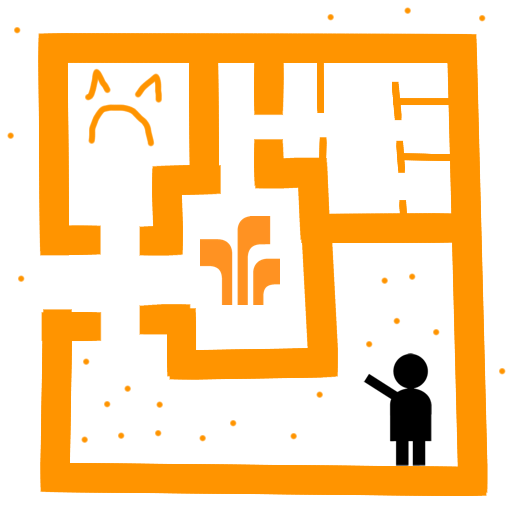
\includegraphics[scale=0.5]{images/test.png}
	\caption{Testgrafik}
	\label{level_1}
\end{figure}
\begin{figure}
	\centering
	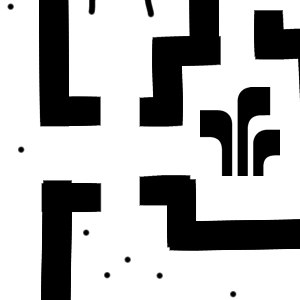
\includegraphics{images/oclusion.png}
	\caption{Oclussionmap}
	\label{o_1}
\end{figure}


\section{Sample Distanz}
Die Oclusionmap wird zur besseren Parallelisierbarkeit in Polarkoordinaten gesampelt.\ref{o_2}
\begin{figure}
	\centering
	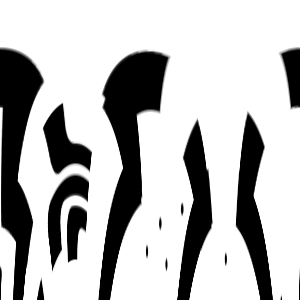
\includegraphics{images/oclusion_polar_2.png}
	\caption{Oclussionmap in polar Koordinaten}
	\label{o_2}
\end{figure}
Nun wird einfach die Distanz für jedes X gemessen bis es auf ein blockierenden Pixel stößt. \ref{o_3}
\begin{figure}
	\centering
	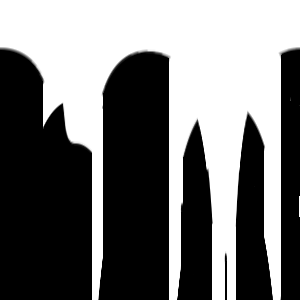
\includegraphics{images/shadow_polar_2.png}
	\caption{Symbolische Shadowmap in polar Koordinaten}
	\label{o_3}
\end{figure}
Die gemessene Distanz wird in einer 1D Textur zur weiter Verarbeitung Gespeichert \ref{o_4}.
\begin{figure}
	\centering
	
\includegraphics[width=0.7\textwidth,height=50px]{images/1DTexture.png}
	\caption{Gesampelte Distanzdaten.}
	\label{o_4}
\end{figure}
\section{Render Licht}
Im letzten Schritt wird ein Sprite in der Größe des lichtes gerendert. Durch Verwendung einer Stepfunktion wird die Distanz zum mittel Punkt mit der maximal Entfernung die in der Textur gespeichert wurde verglichen.
Anschließend muss das Sprite nur noch additiv Geblendet gerendert werden.\ref{level_licht_1}
\begin{figure}
	\centering
	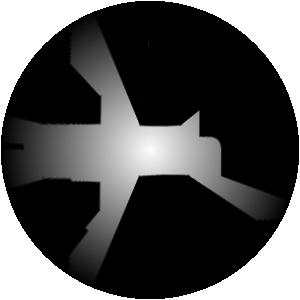
\includegraphics{images/shadow_shadow_2.png}
	\caption{Shadowmap gerendert}
	\label{shadows_1}
\end{figure}
\begin{figure}
	\centering
	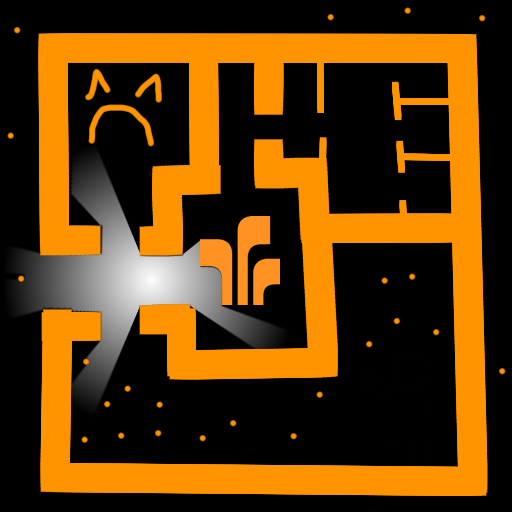
\includegraphics[scale=0.75]{images/final.png}
	\caption{Level mit einem Licht}
	\label{level_licht_1}
\end{figure}